\documentclass{article}
\usepackage[letterpaper,margin=0.5in]{geometry}
\usepackage[sfdefault]{roboto}
\usepackage[T1]{fontenc}
\usepackage[dvipsnames]{xcolor}
\usepackage{tabularx}
\usepackage[shortlabels]{enumitem}
\usepackage{parskip}
\usepackage{incgraph,tikz}
\usepackage{wrapfig}
\usepackage{listings}

\newcommand*{\Ohm}{$\Omega$\ }
\newcommand*{\Indent}{\hspace*{1cm}}
\newcommand*{\Section}[1]{
    \setcounter{subsection}{0}
    \addtocounter{section}{1}
    \addcontentsline{toc}{section}{\protect\numberline{\thesection} #1}
    \Large\textbf{\begin{tabular}{l l}\thesection & #1\end{tabular}}
}
\newcommand*{\Subsection}[1]{
    \setcounter{subsubsection}{0}
    \addtocounter{subsection}{1}
    \addcontentsline{toc}{subsection}{\protect\numberline{\thesubsection} #1}
    \large\textbf{\begin{tabular}{l l}\thesubsection & #1\end{tabular}}
}
\newcommand*{\Header}{
    \rule{\textwidth}{2.5pt}\\
    \begin{tabularx}{\textwidth}{>{\bfseries}l >{\bfseries\centering}X >{\bfseries}r}
    ECEN 3730   & Practical PCB Design \& Manufacture & Professor Tim Swettlten\\
    Spring 2024 & Board 3 Report                      & James K Vogenthaler
    \end{tabularx}\\
    \rule{\textwidth}{1.5pt}

    \vspace*{-5mm}
}

\begin{document}
\setlength\parindent{0pt}
\renewcommand*\contentsname{Table of Contents}

%=============================================================
% Title Page
%=============================================================
\Header

\vspace*{1cm}
\begin{tabularx}{\textwidth}{>{\centering}X}
\Huge \textbf{Golden Arduino}\\
\large A Custom ATMEGA328P Board Design\\
\vspace*{6mm}
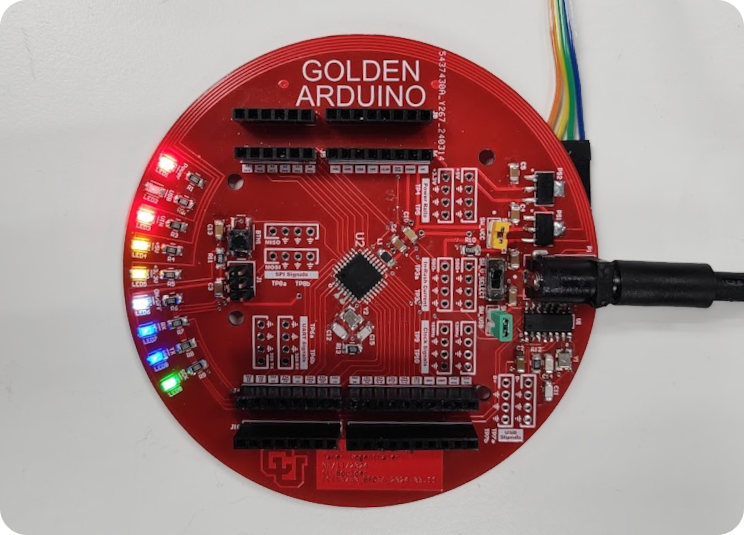
\includegraphics[width=4in]{golden.png}
\vspace*{5mm}
\end{tabularx}

\tableofcontents
\rule{\textwidth}{2.5pt}

\Header

%=============================================================
\section{Plan of Record}
%=============================================================
\subsection{Objective}
The \textit{Golden Arduino} will be a custom redesign of the popular Arduino R3 utilizing best design practices to maximize power and signal integrity (PI/SI).  This entails employing a combination of design choices such as:
\vspace*{2mm}\\
\Indent (1) The placement of decoupling capacitors next to all power pins;\\
\Indent (2) A continuous ground plane to minimize the impedance of return paths;\\
\Indent (3) The placement of ground vias to minimize return paths wherever possible.
\vspace*{2mm}\\
In particular, special attention will paid toward the differences in switching noise and near-field emissions between this board's design and a commercial Arduino R3 board design using a specialized "noise shield" which has been engineered to draw a large amount of current in a short amount of time.

\Indent Finally, features will added expressly for risk mitigation or bring up testing.
A TVS IC will be introduced to protect sensitive components from the effects of electrostatic discharge (ESD).
Additionally, isolation switches, test points, and indicator LEDs will be placed throughout the design to aid in debugging and bring up testing.

%-----------------------------------------
\subsection{Introduction}
%-----------------------------------------
Switching noise is a phenomenon seen along a or between nearby signal traces due to inductive or capactive cross-talk. 

\Indent The first type of noise that this design seeks to mitigate is known as \textit{power rail collapse}, and occurs when there is a sudden draw of current on the power rail.
The change in current over time (dI/dt) that passes through the power rail's parasitic inductance temporarily causes a voltage drop, and similarly a voltage spike can be observed when the current suddenly stops, which is then passed along to any accompanying load.
This type of switching noise can be dramatically reduced through the use of decoupling capacitors to decouple nearby loads from the inductance of the supplying trace.

\Indent The second type of noise this design seeks to mitigate is known as \textit{ground bounce}, and similarly occurs due to changing currents passing through the parasitic inductance of the signal's return path, and can is compounded with each signal that shares this return path. 
This kind of noise can be reduced through the usage of a solid ground plane, which both minimizes the impedance of and distributes the return path of any connected signals.

\Indent Finally, the third type of noise this design seeks to mitigate are the range of \textit{near field emissions} which can extend much farther than intended when there is a large separation between signals and their return paths.
All interconnects will exhibit some near field electromagnetic interference, but their effect can be reduced through the placement of ground vias wherever possible.

%-----------------------------------------
\subsection{Risk Mitigation}
%-----------------------------------------
\begin{itemize}
    \setlength\itemsep{-2mm}
    \item Isolation switches were added along the power rail to enable the troubleshooting of individual design areas.
    \item Filter capacitors to added to the 3.3V and 5V LDOs to prevent higher frequencies from resonating in the feedback loop.
    \item A small amount of capacitance was connected to the crystal oscillators to help jumpstart oscillation.
    \item Test points and LEDs were connected to critical signals to assist in measuring and troubleshooting those signals.
    \item A TVS Diode was connceted to the data lines of the USB to protect that connection from Electrostatic Damage (ESD).
    \item Decoupling capacitors were placed next to all power pins to protect components from power rail collapse.
    \item Ground vias were placed next to all return paths to minimize the effects of ground bounce.
    \item Power traces driving large currents were made much wider to minimize the risk of thermal runway.
\end{itemize}
%-----------------------------------------
\subsection{Component Selection}
%-----------------------------------------
\begin{itemize}
    \setlength\itemsep{-2mm}
    \item ATMEGA328P-AU (Arduino Microcontroller)
    \item CH340G (USB to Serial Bridge)
    \item 5.0V and 3.3V LDO (Low Dropout Regulators)
    \item 16MHz and 12MHz Crystal Oscillators
    \item SRV05-4-P-T7 TVS (Diode Voltage Regulator)
\end{itemize}

\igrset{paper=letter, landscape, options={width=10.5in}, bookmark options={level=subsection}}

%=============================================================
% Design and Assembly
%=============================================================
\incgraph[top border=1cm, overlay={
    \node at ([xshift=4cm, yshift=-1cm]page.north west) {\Section{Design and Assembly}};
    \node at ([xshift=2.7cm, yshift=-2cm]page.north west) {\Subsection{Schematic}};
    \node at ([yshift=1cm]page.south) {\thepage};
}]{schematic.png}

\Header

\vspace*{5mm}
\Subsection{Layout}\\
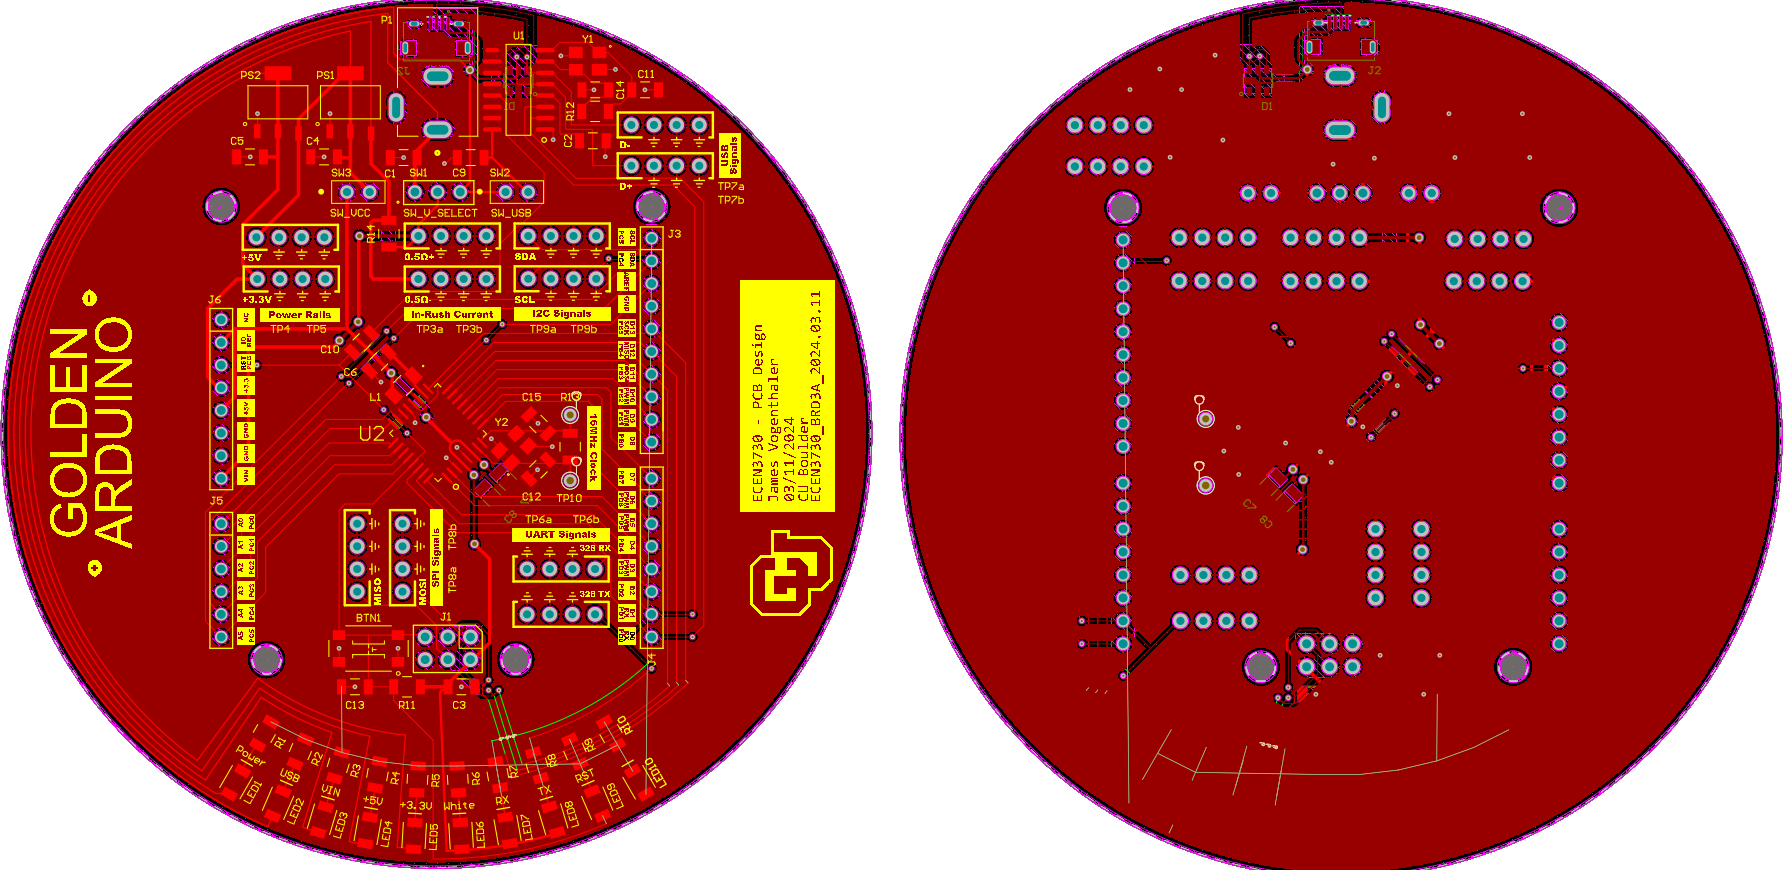
\includegraphics[width=\textwidth]{layout.png}

\vspace*{5mm}
\Subsection{Assembly}\\
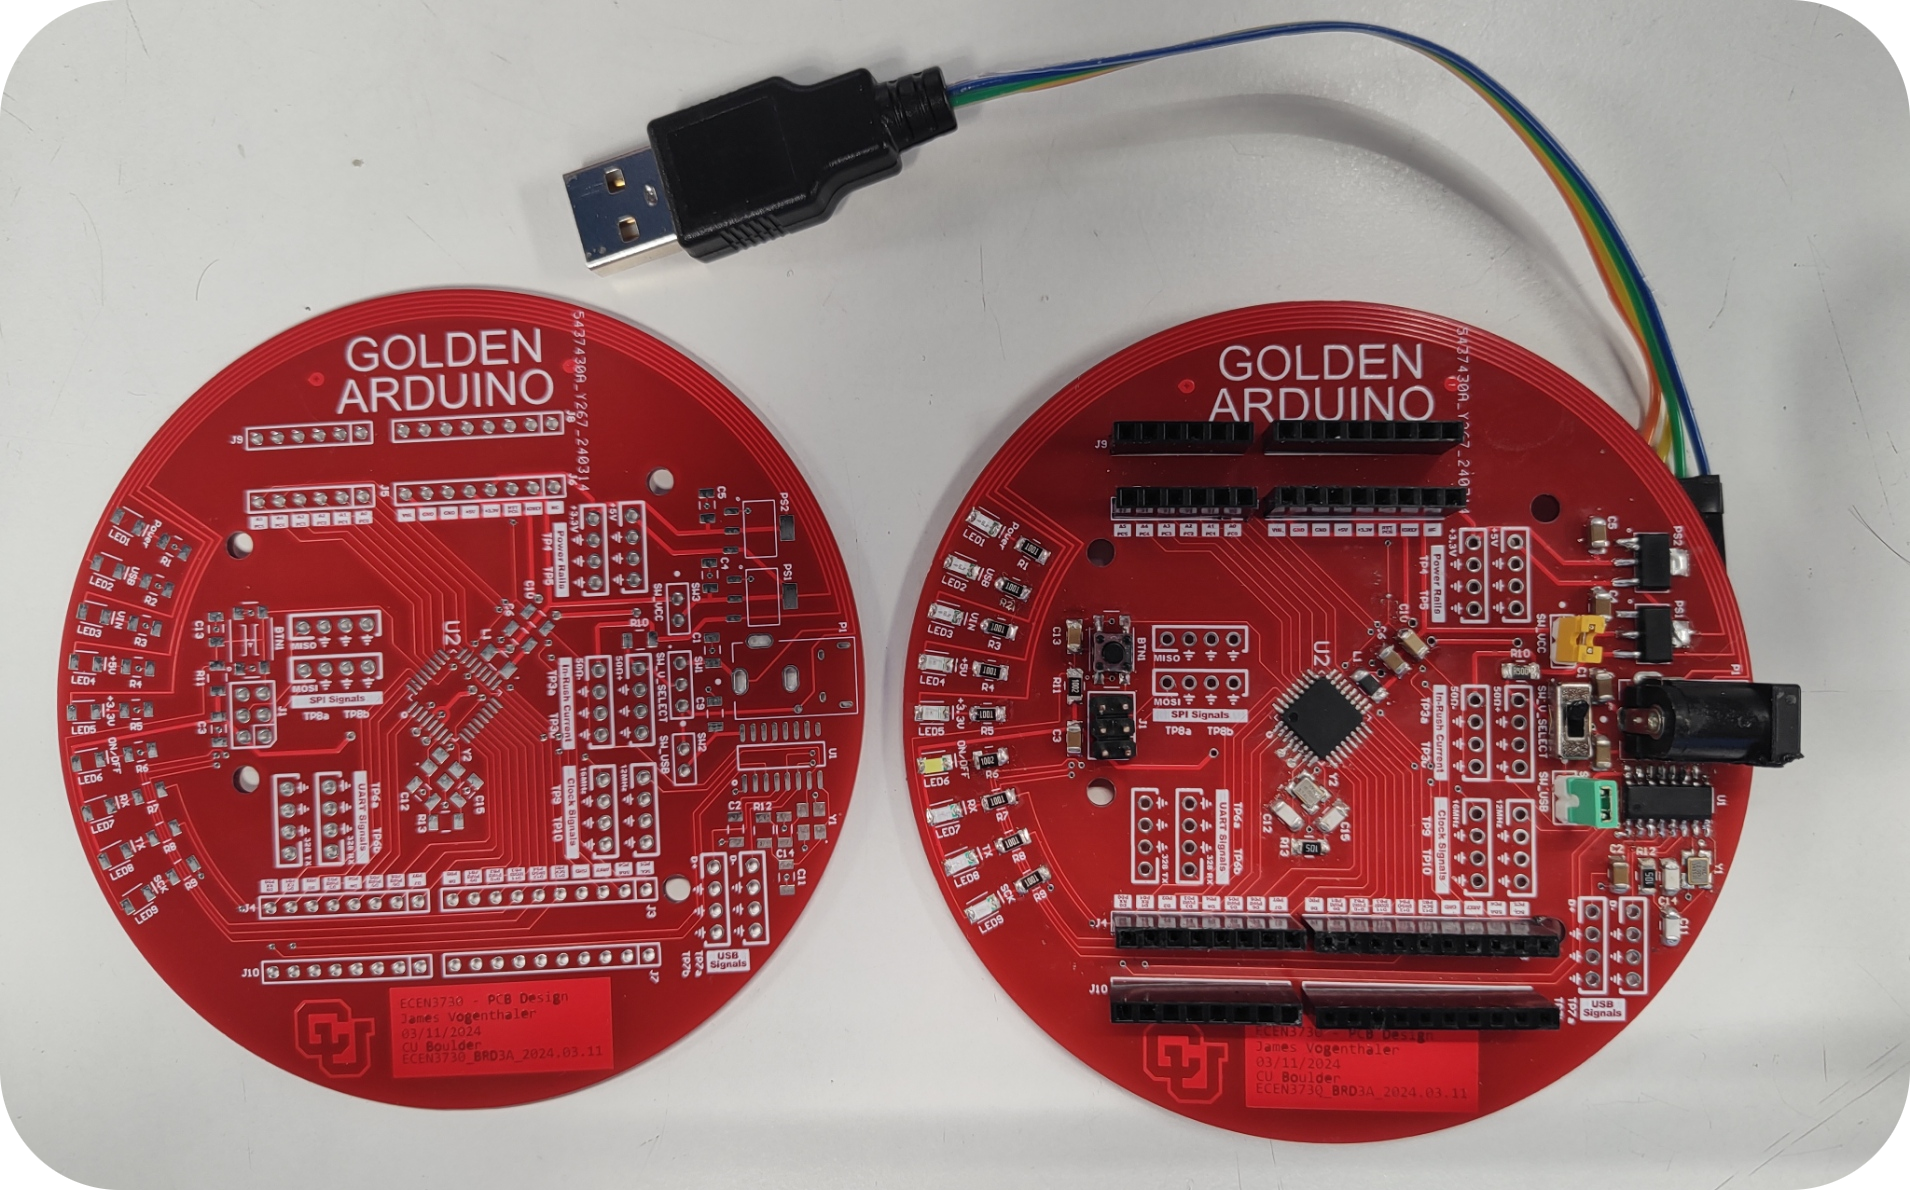
\includegraphics[width=\textwidth]{assembled.png}

%=============================================================
\Header

\begin{wrapfigure}{r}{3in}
    \vspace*{-2.0cm}
    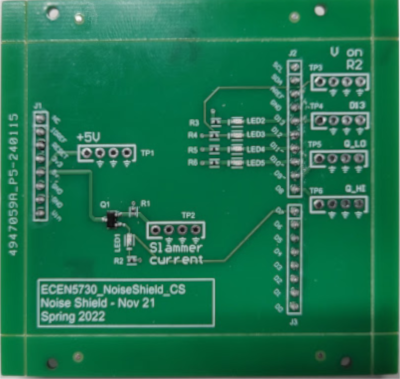
\includegraphics[width=3in]{shield.png}
    \caption{Specialized Noise Shield}

    \vspace*{0.5cm}
    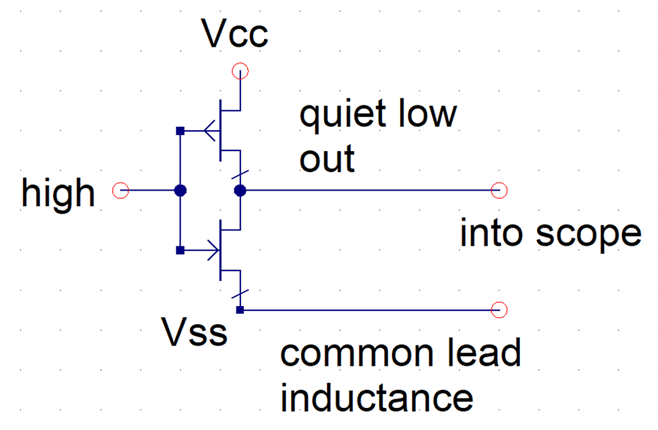
\includegraphics[width=3in]{quiet.png}
    \caption{Quiet Low Diagram}
    \vspace*{-1.5cm}
\end{wrapfigure}

%=============================================================
\section{Bring Up and Testing}
%=============================================================
\subsection{Noise shield}
For this lab, a noise shield was provided which allowed for the simulatenous switching of several outputs which all draw high current.
This shield will be used to test the magnitude of switching noise and range of near-field emissions on both the custom design and a commercial Arduino Uno R3 for comparison.

%-----------------------------------------
\subsection{Experiment Description}
%-----------------------------------------
The following 3 experiments were performed w/ this shield:
\begin{enumerate}[(a)]
    \item \textbf{Switching I/O:} Digital pins D10, D11, D12, and D13 were repeatedly switched on and off. Pins 10 through 12 are each driving an LED and a 47\Ohm resistor to draw a large amount of current. Pin 13 drives a 1k\Ohm resistor and an LED, and is used to trigger the scope. Pins 8 and 9 are driven at a constant value; since they're output is controlled by a transistor, this effectively connects them to the on-chip VCC and GND rails of the ATMEGA328P uC.

    \Indent Test points are connected to Pin 8 and 9 so that we can observe the effect of the large changes in current in the nearby aggressor traces on the quiet high and low signals. Since pin 9 is routed closer to the aggressor lines, we should expect to see a larger effect on our quiet low signal. A test point is added across the 47\Ohm reisistor of Pin 12 to help measure current.
\end{enumerate}

\begin{enumerate}[(b)]
    \item \textbf{Slammer Circuit:} Digital pin 7 is connected to an N-channel MOSFET to act as a relay for the current flowing through a 10\Ohm resistor. Since this resistor would otherwise be directly connected to the on-board 5V rail, we can expect around 400-500 mA of current to flow through this resistor, which means extra care must be taken to limit the amount of time this resistor is active as a safety consideration.  A test point is connected directly to the on-board 5V rail at the collector pin of the FET. Since there is no decoupling capacitor here, we should expect to observe the effects of \textit{power rail collapse} or a voltage droop when the current is switched on, and a voltage spike when switched off.
\end{enumerate}

\begin{enumerate}[(c)]
    \item \textbf{Loop-to-loop Crosstalk:} If we take a 10x probe with the tip shorted to its own ground rail through a small loop, we can effectively use it as an antenna to measure the strength of near-field emissions around the device under test (DUT). Since we wish to measure the electromagnetic interference coming from the board and not the shield, the \textit{scope antenna} will be used to scan the area underneath the board until the highest point of noise is found.
    
    \Indent If the near-field emissions coming off of the board are too large in magnitude, they are then considered \textit{far-field emissions} and can begin to affect surrounding devices and even fail FCC certification tests.
\end{enumerate}

\Header

%-----------------------------------------
\subsection{Bootloading}
%-----------------------------------------
Initially, there were issues bootloading the ATMEGA328P uC due to incorrect capacitor values being used between the reset pin of the 328 and the DTR pin of the CH340G, as well as for the reset button's debouncing capacitor. This prevented the 328 from receiving the reset signals from the in-circuit serial programmer properly. This has since been corrected on the design and layout.

\Indent Once bootloaded, both the UART (TX/RX) pins and the Arduino itself was testing using the example blink program. The blink program was then modified to phase through brightness levels to look like a heartbeat in order to ensure that the logic on the chip itself was working properly. Once successfully bootloaded, the noise shield could be tested using the code below:

%-----------------------------------------
\subsection{Noise Shield Driver Code}
%-----------------------------------------
\begin{lstlisting}[language=c]
    void setup() { 
        DDRB = B00111111;       // Set pins 8 through 13 as OUTPUT pins
        pinMode(7, OUTPUT);     // Set pin 7 as an OUTPUT pin
        PORTB = B00000001;      // Set pin 8 Quiet High & 9 Quiet Low
        digitalWrite(7, LOW);   // Ensure slammer circuit starts off
    } 
    void switching_io() {       // Function for switching D10-13 on/off
        PORTB = B00111101;      
        delayMicroseconds(4); 
        PORTB = B00000001; 
        delay(1); 
    }
    void slammer() {            // Function for controlling slammer circuit
        digitalWrite(7, HIGH); 
        delayMicroseconds(400); 
        digitalWrite(7, LOW); 
        delay(10); 
    }
    void loop() {               // Only use either switching I/O or
        switching_io();         // slammer to ensure consistent timing
        // slammer();           // for the oscilloscope trigger
    }
\end{lstlisting}

%-----------------------------------------
\subsection{Measuring Mutual Aggression}
%-----------------------------------------

%-----------------------------------------
\subsection{Measuring Self Aggression}
%-----------------------------------------

%-----------------------------------------
\subsection{Measuring Near-Field Emissions}
%-----------------------------------------

%-----------------------------------------
\subsection{Measuring Peak In-rush Current}
%-----------------------------------------

%=============================================================
\section{Analysis \& Conclusions}
%=============================================================
\subsection{Performance Comparison}
\Indent The custom ATMEGA328P board design far outperformed the commercial Arduino R3 model in terms of noise reduction, near-field emission levels, and signal integrity. This is very much a result of having followed best design practices discussed above to limit the noise produced by ground bounce and parasitic inductance. As shown in figure x, the commercial Arduino features many more cross unders and . 

%-----------------------------------------
\subsection{What worked well?}
%-----------------------------------------
\Indent The circular design actually lended itself to a more fluid design that wasn't constrained by 90 degree or 45 degree angles. An online graphing tool called $Desmos$ was used to quickly calculate the position and rotation of various components such as the LEDs based on a desired radius and angle from the center of the design. In the future, I am considering developing an Altium extension to make the placement of components using polar coordinates an option because of how well this design worked.

\Indent Also, as is clear from the performance comparison, is how effective the usage of the best design practices were. The Golden Arduino design far outperformed the commercial board in terms of signal integrity and near-field emissions.

%-----------------------------------------
\subsection{What didn't work?}
%-----------------------------------------
\Indent There were several mistakes in the design that made assembly somewhat difficult. Particularly the incorrect capacitance values for the components connecting to the reset pin. Additionally, the USB port was accidentally placed backwards on the board layout, and a USB Type A had to be manually soldered onto the respective USB signal traces. In the future, this can be solved by paying extra special attention to critical components such as the reset signal and the usb component. The quick inspection of the components in the layout using the 3D preview feature in Altium could've also helped to catch the backwards placement of the USB connector.

\Indent Additionally, the commercial Arduino R3 board also demonstrated lower on-board power-rail noise than the Golden Arduino design during the slammer circuit experiment. This is likely because there were no decoupling capacitors placed next to the 3.3V and 5V output header pins, and really demonstrates how much power integrity depends on the usage of decoupling capacitors. Future iterations of this board will include decoupling capacitors adjacent to any output power pins.

\Indent Another pitfall was the 3-pin switch used to select between voltage sources. While convenient, the cheap construction of the switch actually causes a very short connection between all three pins during transition, which could have potentially disasterous effects. In the future, either a more expensive 3-pin switch should be used, or a 2-pin connector should be used to toggle between sources on the 3-pin connection instead.

%-----------------------------------------
\subsection{Takeaway}
%-----------------------------------------
\Indent Overall, this design and the accompanying experiments truly showcase the benefits of following best design practices, as is evident in the performance comparison. In particular, the usage of a continuous ground plane, decoupling capacitors, ground vias next to all return paths, and the separation of critical signals from high frequency traces are especially effective methods for reducing the noise seen in a design. The best part about following these best design practices is that they often take minimal effort and add little to no cost to a design, and so simply following them enables for increased performance at no extra cost.

\Indent Another key takeaway is the need for careful review of a design before sending it off for production or manufacturing, as the reversed placement of the USB port signficantly increased the challenges associated with bringing up this board design. In fact, any kind of risk reduction can help to avoid problems such as these, and the challenges faced in this experiment showcase exactly that.

\end{document}
